\chapter{專題背景和動機}
\renewcommand{\baselinestretch}{10.0} %設定行距
\pagenumbering{arabic} %設定頁號阿拉伯數字
\setcounter{page}{1}  %設定頁數
\fontsize{14pt}{2.5pt}\sectionef
\section{研究動機}

高中職到大學現在所教的繪圖軟體都是老師在業界中所挑選出來的,不外乎最主要的軟體就是 Soidworks ,身為業界中中小企業最受歡迎的程式,只要是有畫 3D 繪圖的人都一定知道的,但在專題老師的介紹下,我們得知了不輸於 Solidworks 的繪圖軟體 Solid Edge 以及同公司旗下的限元素分析軟體 Femap 。 Solidworks 在台灣機械領域已經有個不可動搖的地位存在了,但我們必須讓這些不亞於 SW 的優良軟體浮出水面,讓更多的人知道不是只要學會 Solidworks 就行了!\\
\begin{figure}[hbt!]
\begin{center}
\includegraphics[angle=90,width=10cm]{}
\caption{\Large }\label{fig.}
\end{center}
\end{figure}
\begin{figure}[hbt!]
\begin{center}
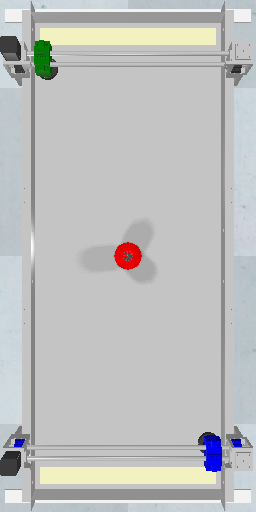
\includegraphics[angle=90,width=10cm]{origin}
\caption{\Large }\label{fig.}
\end{center}
\end{figure}
\begin{figure}[hbt!]
\begin{center}
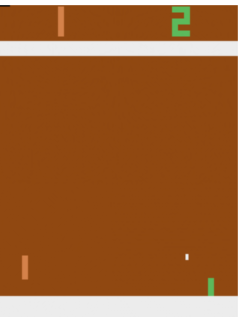
\includegraphics[height=8cm]{pong_gym}
\caption{\}\label{fig.}
\end{center}
\end{figure}
\section{ Solid Edge 簡介}
 Solid Edge 是一個完整的混合式 2D/3D CAD 系統,從零件、組裝、工程圖等研發工作流程一次完成。並搭載 Siemens 獨家 同步建模技術 ,能夠加速設計、更快的設計變更、提高匯入資料重用效率。

同步建模技術結合了速度和靈活性,直接建模,控制精確的尺寸驅動設計(功能和同步解決相關的參數)。參數的關係,可直接應用於固體功能,而不必依賴於二維草圖幾何關係和共同參數自動應用。該建模過程是表示要爭取一定的 CAD 設計活動高達100倍的速度。

不像其他直接建模系統,它不是典型的帶動歷史的建模方法,而不是提供參數化尺寸驅動的建模幾何通過同步,參數和使用規則的決策引擎,讓用戶使用不可預測的變化。這個對象驅動的編輯模式是被稱為對象操作界面,它強調一個用戶界面,提供直接操縱的對象( DMUI )。

2007年, SIEMENS (西門子股份有限公司)工業自動化部門收購了 UGS 公司,後將 UGS 的公司更名為 Siemens PLM Software 。 \\
\section{ Femap 簡介}
 Femap 是一種嵌入在 Siemens PLM Software 的分析軟體,它提供了一個循序漸進的方法,以單個組件的分析建立 CAD 軟件系統的 Solid Edge CAD 解決方案,其成本低廉的高性能 FEA 建模,也適合工程師使用。 Femap 公認為全球領先獨立的 CAE 前後處理器,可用於進階工程有限元素分析,可以快速、輕鬆地確定過程中的組件是否滿足強度要求。 \\
 
\begin{enumerate}
\item 
\item 
\item 
\end{enumerate}

\renewcommand{\baselinestretch}{0.5} %設定行距
